Архитектура кодировщик-декодировщик широко распространена в машинном обучении, теории кодирования, компрессии и
криптографии. Нейросети также используют этот подход для задач \begin{itemize}
    \item генерации перевода и пересказа
    \item классификации текста
    \item распознания частей речи и выделения имен собственных
\end{itemize}

\begin{figure}[h]
    \centering
    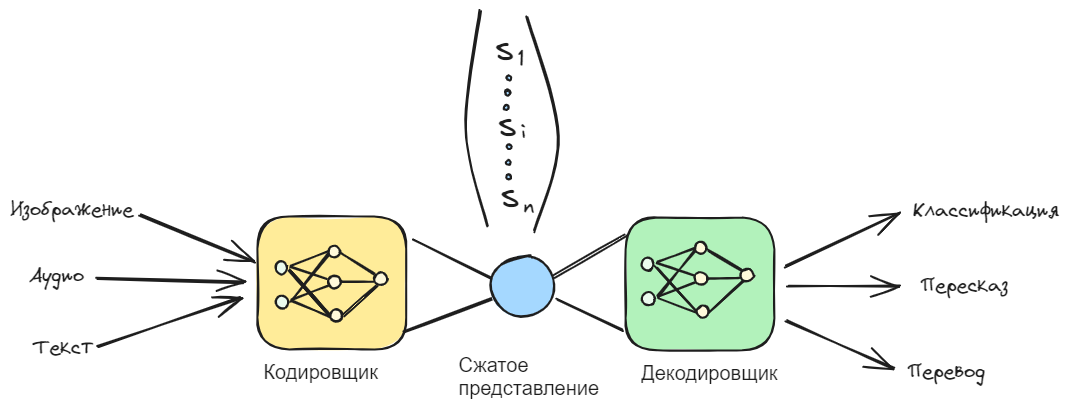
\includegraphics[width=0.5\textwidth]{assets/ml/nn/encoder_decoder.excalidraw.png}
    \caption{Преобразование сигнала выполняется в промежуточных слоях активации в ходе прямого распространения сигнала}
    \label{encoder}
\end{figure}

Такая архитектура 

\textit{Определение} Рекуррентными нейронными сетями называют
называется слои, использующие предыдущие скрытые состояния для расчета следующих.
\begin{equation}
    \begin{aligned}
        & h_t = \sigma (W_x x_t + W_h h_{t-1}+ b_h) \\
        & y_t = \sigma (W_y h_t + b_y), где \\
    \end{aligned}
\end{equation}
где \begin{itemize}
    \item $x_t$, $h_t$, $y_t$ векторы входного, скрытого и выходного слоя
    \item $W_x$, $W_h$, $W_y$ матрицы обновления состояния.
\end{itemize}
\begin{figure}[h]
    \centering
    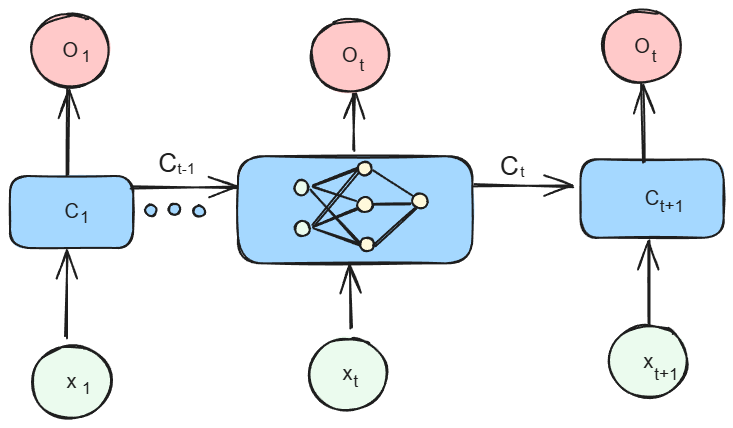
\includegraphics[width=0.5\textwidth]{assets/ml/nn/rnn.excalidraw.png}
    \caption{Каждая ячейка рекуретной нейронной сети выполняет обновление представления.}
    \label{reccurent}
\end{figure}
Ошибка модели для случая обработки последовательностей 
одинаковой длины запишется как:
\begin{equation}
    \mathcal{L}(\hat{y},y) = \sum_{t=1}^{T_y} \mathcal{L}(\hat{y},y)
\end{equation}
На практике матрицы обновления постоянные для каждой ячейки, поэтому
правило обновления матрицы весов $W$ запишется как:
\begin{equation}
    \frac{\partial \mathcal{L}^{(T)}}{\partial W} = \sum_{t=1}^T \frac{\partial \mathcal{L}^{(T)} }{\partial W}
\end{equation}
Такой подход называется распространением ошибки во времени. 
Также существуют модификации механизма нейронной сети
заключающие в добавлении параллельного блока памяти \begin{itemize}
    \item Долгая короткая память \cite{ochreiter1997long}
    \item Управляемый рекуррентный блок \cite{chung2014empirical}
\end{itemize}

Механизм внимания, основанный на модели рабочей памяти моделей рабочей памяти \cite{wallace1960plans},
позволил значительно улучшить результаты
задач перевода, пересказ и понимания языка \cite{bahdanau2014neural}.
Механизм внимания вычисляет вектор внимания \( \alpha \),
который определяет важность каждого элемента входной последовательности
на текущем временном шаге \cite{bahdanau2014neural}:
\begin{equation}
    \alpha_t = \text{softmax}(f(h_t, X))
\end{equation}
где \( f \) - функция, которая вычисляет важность каждого элемента входной последовательности, а \( \text{softmax} \) применяется для получения нормированных весов внимания.

\begin{figure}[h]
    \centering
    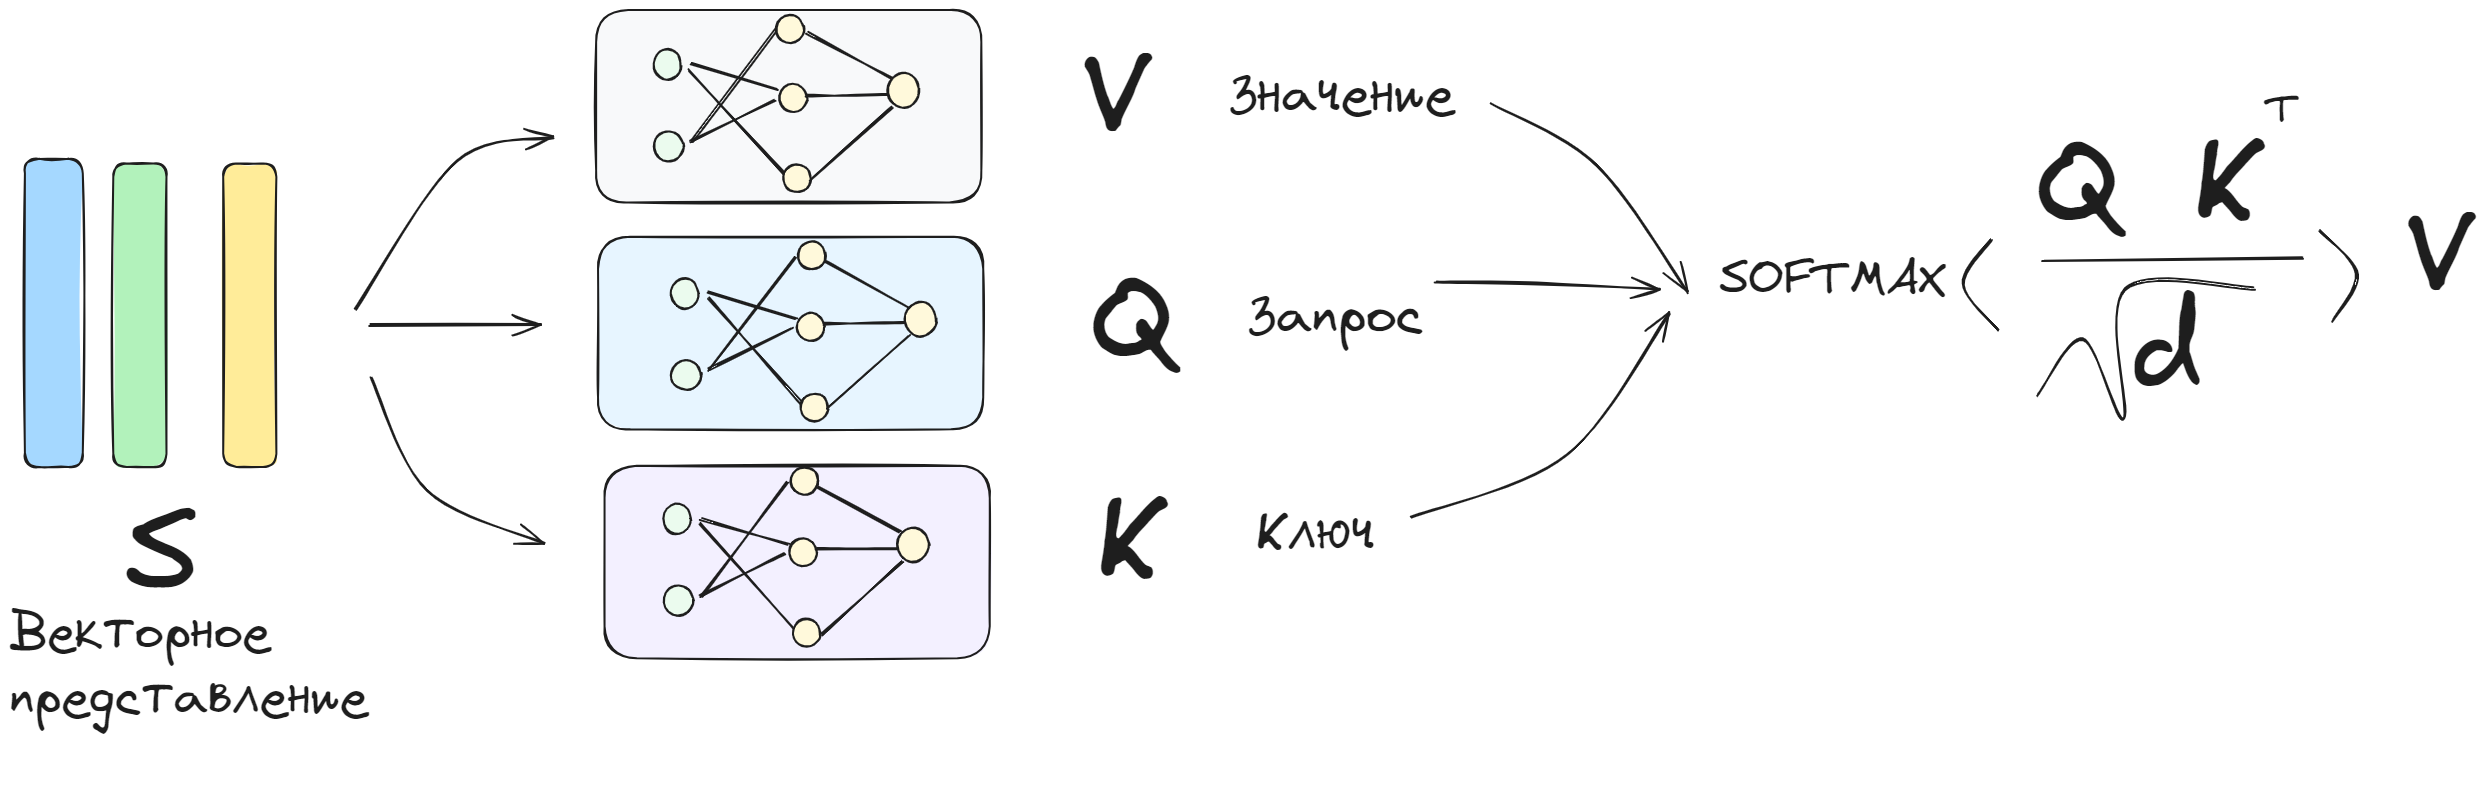
\includegraphics[width=0.5\textwidth]{assets/ml/nn/attention.excalidraw.png}
    \caption{Механизм внимания в архитектуре Transformer (Self Attention) \cite{vaswani2017attention} }
    \label{self_attention}
\end{figure}

Механизм внимания позволяет модели сосредоточиться на наиболее значимых частях входных данных в каждый момент времени, что делает его особенно полезным для задач, 
требующих адаптивности и контекстного понимания, таких как машинный перевод, генерация текста и вопросно-ответные системы. 
Этот механизм стал ключевым инструментом в области генеративного моделирования естественного языка, позволяя моделям эффективно работать с различными типами данных и контекстами.

